\documentclass[11pt]{article}
\usepackage[margin=0.5in,top=0.8in,bottom=0.8in]{geometry}
\usepackage{graphicx,amsmath}

\newcommand{\beq}{\begin{equation}}
\newcommand{\eeq}{\end{equation}}
\newcommand{\beqn}{\begin{eqnarray}}
\newcommand{\eeqn}{\end{eqnarray}}
\newcommand{\ve}[1]{\mbox{\boldmath $#1$}}
\newcommand{\la}{\stackrel{<}{ _{\sim}}}

\begin{document}

\begin{center}
{\huge {\bf Linear Regression Demystified}}

{\large Yuk Tung Liu}
\end{center}

\bigskip

Linear regression is an important subject in statistics. In elementary 
statistics courses, formulae related to linear regression are often 
stated without derivation. Here I derive these formulae 
for students with more advanced math background.  

\section{Simple Regression: One Variable}

\subsection{Least Square Prescription}

Suppose we have a set of data points $(x_i,y_i)$ ($i=1,2,\cdots,n$). The 
goal of linear regression is to find a straight line that best fit the data. 
In other words, we want to build a model 
\beq
  \hat{y}_i = \beta_0 + \beta_1 x_i 
\label{def:yhat}
\eeq 
and tune the parameters $\beta_0$ and $\beta_1$ so that $\hat{y}_i$ is as 
close to $y_i$ as possible for all $i=1,2,\cdots,n$.

Before we do the math, we need to clarify the problem. How do we judge the 
``closeness'' of $\hat{y}_i$ and $y_i$ for all $i$? If the data points 
$(x_i,y_i)$ do not fall exactly on a straight line, $y_i$ and $\hat{y}_i$ 
is not going to be the same for all $i$. The deviation of $y_i$ from 
$\hat{y}_i$ is called the {\it residual} and is denoted by $\epsilon_i$ 
here. In other words, 
\beq
  y_i = \hat{y}_i + \epsilon_i = \beta_0 + \beta_1 x_i + \epsilon_i  .
\label{def:residual}
\eeq
The least square prescription is to find $\beta_0$ and $\beta_1$ that 
minimize the sum of the square of the residuals $SSE$: 
\beq
  SSE = \sum_{i=1}^n \epsilon_i^2 = \sum_{i=1}^n (y_i-\hat{y}_i)^2 
= \sum_{i=1}^n (y_i-\beta_0-\beta_1 x_i)^2 .
\label{def:SSE}
\eeq
If you are familiar with calculus, you will know that the minimization can be 
done by setting the derivatives of $SSE$ with respect to $\beta_0$ and 
$\beta_1$ to 0, i.e.\ $\partial SSE/\partial \beta_0 =0$ and 
$\partial SSE/\partial \beta_1=0$. The resulting equations 
are\footnote{Careful students may realize 
that this only gaurantees that $SSE$ is stationary but not necessarily minimum. There is also 
a concern whether the resulting solution is a global minimum or a local minimum. Detail 
analysis (see Section~\ref{sec:regeq}) reveals that the solution in our case is a global minimum.}  
\beq
  \sum_{i=1}^n (y_i-\hat{y}_i) = \sum_{i=1}^n \epsilon_i = 0 \ \ \ \mbox{ and } \ \ \ 
  \sum_{i=1}^n x_i (y_i-\hat{y}_i) = \sum_{i=1}^n x_i \epsilon_i = 0 .
\label{eq:regeqs0}
\eeq
We can combine the first and second equation to derive an alternative equation for 
the second equation: 
\[
  \sum_{i=1}^n \epsilon_i = 0 \ \ \Rightarrow \ \ 
  \sum_{i=1}^n \bar{x} \epsilon_i = 0 
\]
Subtracting this equation from the second equation of (\ref{eq:regeqs0}) yields 
\[
  \sum_{i=1}^n (x_i-\bar{x}) \epsilon_i = 0 .
\]
Equation~(\ref{eq:regeqs0}) can be expressed as 
\beq
  \sum_{i=1}^n (y_i-\hat{y}_i) = \sum_{i=1}^n \epsilon_i = 0 \ \ \ \mbox{ and } \ \ \ 
  \sum_{i=1}^n (x_i-\bar{x}) (y_i-\hat{y}_i) = \sum_{i=1}^n (x_i-\bar{x}) \epsilon_i = 0 .
\label{eq:regeqs}
\eeq

If you are not familiar with calculus, I can show you a proof using algebra. 
I actually prefer that proof since it is more rigorous. Before presenting the 
proof, let's remind you some concepts in statistics. 

\subsection{Mean, Standard Deviation and Correlation}

The mean and standard deviation of a set of points $\{ u_i\}$ are defined as
\beq
  \bar{u} = \frac{1}{n} \sum_{i=1}^n u_i \ \ \ , \ \ \
  SD_u = \sqrt{ \frac{1}{n} \sum_{i=1}^n (u_i-\bar{u})^2 }  \ .
\label{def:mean_std}
\eeq
The $Z$ score of $u_i$ is defined as
\beq
  Z_{u i} = \frac{u_i-\bar{u}}{SD_u} .
\label{def:Zscore}
\eeq
The {\it correlation} of two set of points (with equal number of elements) $\{ x_i \}$
and $\{ y_i \}$ is defined as
\beq
  r_{xy} = r_{yx} = \frac{1}{n} \sum_{i=1}^n Z_{xi} Z_{yi}  
= \frac{1}{n} \sum_{i=1}^n \frac{(x_i-\bar{x})(y_i-\bar{y})}{SD_x SD_y}
\label{def:correlation}
\eeq
The Cauchy-Schwarz inequality states that for two set of real numbers $\{ u_i\}$ 
and $\{ v_i \}$, 
\[
  \left( \sum_{i=1}^n u_i v_i \right)^2 \leq \left( \sum_{i=1}^n u_i^2\right) 
\left( \sum_{i=1}^n v_i^2 \right) 
\]
and the equality holds if and only if $v_i=k u_i$ for all $i$, where $k$ is 
a constant. You can find the proof of the inequality in, e.g., Wikipedia.

It follows from the Cauchy-Schwarz inequality that the correlation 
$|r_{xy}| \leq 1$, with $|r_{xy}|=1$ if and only if $x_i$ and $y_i$ fall 
exactly on a straight line, i.e.\ $\epsilon_i=0$ for all $i$. So 
the correlation $r_{xy}$ measures how tightly the points $(x_i,y_i)$ are clustered 
around a line.

\subsection{Regression Equation}
\label{sec:regeq}

To derive the regression equation, we first rewrite $SSE$ in equation~(\ref{def:SSE}) 
in terms of Z-scores. It follows from the definition of Z-scores that 
\[
  x_i = \bar{x} + SD_x Z_{xi} \ \ \ , \ \ \ y_i = \bar{y} + SD_y Z_{yi} 
\]
and the $SSE$ becomes 
\beqn
  SSE &=& \sum_{i=1}^n [\bar{y} + SD_y Z_{yi} - \beta_0 - \beta_1 (\bar{x} + SD_x Z_{xi}) ]^2 \cr 
\cr
&=& \sum_{i=1}^n (SD_y Z_{yi} - \beta_1 SD_x Z_{xi} + \bar{y}-\beta_0 -\beta_1 \bar{x})^2 \nonumber
\eeqn
For simplicity, we denote $\tilde{\beta}_0 = \bar{y}-\beta_0 -\beta_1 \bar{x}$. Then we have 
\beqn
  SSE &=& \sum_{i=1}^n (SD_y Z_{yi} - \beta_1 SD_x Z_{xi} + \tilde{\beta}_0)^2 \cr \cr 
&=& SD_y^2 \sum_{i=1}^n Z_{yi}^2 + \beta_1^2 SD_x^2 \sum_{i=1}^n Z_{xi}^2 
+ \sum_{i=1}^n \tilde{\beta}_0^2 -2\beta_1 SD_x SD_y \sum_{i=1}^n Z_{xi} Z_{yi} \cr \cr 
&& + 2\tilde{\beta}_0 SD_y \sum_{i=1}^n Z_{yi} 
- 2\tilde{\beta}_0 \beta_1 SD_x \sum_{i=1}^n Z_{xi} 
\label{eq:SSEtmp0}
\eeqn
Recall that the Z-scores are constructed to have zero mean and unit standard deviation. 
It follows that 
\[
  \sum_{i=1}^n Z_{xi}=\sum_i Z_{yi} = 0  \ \ , \ \ \frac{1}{n} \sum_{i=1}^n Z_{xi}^2 
= \frac{1}{n} \sum_{i=1}^n Z_{yi}^2 = 1 
\]
and from the definition of correlation we have 
\[
  \frac{1}{n} \sum_{i=1}^n Z_{xi} Z_{yi} = r_{xy} ,
\]
Thus the SSE in equation~(\ref{eq:SSEtmp0}) can be written as 
\beqn
  SSE &=& n (SD_y^2 + \beta_1^2 SD_x^2 + \tilde{\beta}_0^2 - 2\beta_1 r_{xy} SD_x SD_y) \cr
&=& n [ \tilde{\beta}_0^2 + (SD_x \beta_1 - r_{xy} SD_y)^2 + (1-r_{xy}^2)SD_y^2 ] \cr
&=& n [ (\bar{y}-\beta_0 -\beta_1 \bar{x})^2 + (SD_x \beta_1 - r_{xy} SD_y)^2] + n(1-r_{xy}^2)SD_y^2 
\label{eq:SSEgen}
\eeqn
Note that we have re-expressed $\tilde{\beta}_0$ in terms of $\beta_0$ and $\beta_1$ in 
the last step. Remember our goal is to find $\beta_0$ and $\beta_1$ to minimize 
$SSE$. The quantity inside the square bracket in equation~(\ref{eq:SSEgen}) is 
a sum of two squares and contain the variables $\beta_0$ and $\beta_1$, whereas 
$n(1-r_{xy}^2)SD_y^2$ is a fixed quantity. Therefore, we conclude that 
\[
  SSE \geq n(1-r_{xy}^2)SD_y^2
\]
and the equality holds if and only if 
\[
 \bar{y}-\beta_0 -\beta_1 \bar{x} = 0 \ \ \mbox{ and } \ \ 
  SD_x \beta_1 - r_{xy} SD_y = 0 .
\]
Therefore, the values of $\beta_0$ and $\beta_1$ that minimize $SSE$ is 
\beq
  \boxed{ \beta_1 = r_{xy} \frac{SD_y}{SD_x} \ \ , \ \ \beta_0 = \bar{y}-\beta_1 \bar{x} }
\label{eq:regcoefs0}
\eeq
and the minimum $SSE$ is 
\beq
  \boxed{ SSE = n(1-r_{xy}^2) SD_y^2 }
\label{eq:SSEmin}
\eeq

How are equations~(\ref{eq:regcoefs0}) related to equations~(\ref{eq:regeqs}) derived 
from calculus? We are going to prove that they are the same thing. 
Using equations~(\ref{eq:regcoefs0}) we have 
\beqn
  \sum_{i=1}^n \epsilon_i  &=& \sum_{i=1}^n (y_i - \hat{y}_i) \cr \cr 
&=& \sum_{i=1}^n (y_i - \beta_0 - \beta_1 x_i) \cr \cr 
&=& \sum_{i=1}^n (y_i - \bar{y} + \beta_1 \bar{x} - \beta_1 x_i) \cr \cr 
&=& \sum_{i=1}^n (y_i - \bar{y}) - \beta_1 \sum_{i=1}^n (x_i-\bar{x}) \cr \cr 
&=& 0 \nonumber 
\eeqn
If the last step is not obvious to you, here's a simple proof: 
\[
  \bar{x} = \frac{1}{n}\sum_{i=1}^n x_i \ \ \ \Rightarrow \ \ \ 
  \sum_{i=1}^n x_i = n \bar{x} = \sum_{i=1}^n \bar{x} \ \ \ \Rightarrow \ \ \ 
  \sum_{i=1}^n (x_i-\bar{x}) = 0 
\]
and similarly 
\[
  \sum_{i=1}^n (y_i-\bar{y}) = 0.
\]
Now let's look at the second equation of~(\ref{eq:regeqs}): 
\beqn
  \sum_{i=1}^n (x_i-\bar{x})(y_i-\hat{y}_i) &=& \sum_{i=1}^n (x_i-\bar{x})(y_i-\beta_0-\beta_1 x_i)\cr \cr 
&=& 
\sum_{i=1}^n 
(x_i-\bar{x})(y_i - \bar{y} + \beta_1 \bar{x} - \beta_1 x_i) \cr \cr 
&=& \sum_{i=1}^n (x_i-\bar{x})(y_i - \bar{y}) - \beta_1 \sum_{i=1}^n (x_i-\bar{x})^2 
\nonumber
\eeqn
From the definition of correlation and standard deviation, we have 
\[
  r_{xy} = \frac{1}{n} \sum_{i=1}^n \frac{(x_i-\bar{x})(y_i - \bar{y})}{SD_x SD_y} 
 \ \ \Rightarrow \ \ \sum_{i=1}^n (x_i-\bar{x})(y_i - \bar{y}) = n r_{xy} SD_x SD_y 
\]
\[
  SD_x^2 = \frac{1}{n} \sum_{i=1}^n (x_i-\bar{x})^2 \ \ \Rightarrow \ \ 
\sum_{i=1}^n (x_i-\bar{x})^2 = n SD_x^2 
\]
Thus, 
\[
  \sum_{i=1}^n (x_i-\bar{x})(y_i-\hat{y}_i) = nr_{xy}SD_x SD_y - \beta_1 n SD_x^2 
= n SD_x^2 \left( r_{xy} \frac{SD_y}{SD_x} - \beta_1 \right) = 0.
\]
Therefore, we have proved that equations~(\ref{eq:regeqs}) follows from 
equations~(\ref{eq:regcoefs0}). On the other hand, equations~(\ref{eq:regeqs}) 
are two linear equations for $\beta_0$ and $\beta_1$. We can solve for 
$\beta_0$ and $\beta_1$ from these equations, which we will do so in 
Section~\ref{sec:regcoefs}. 
The result is that $\beta_0$ and $\beta_1$ are given by equations~(\ref{eq:regcoefs0}) 
and so the two sets of equations are equivalent. 

\subsection{Interpretation}

I will try to give you an intuition of the meaning of equations~(\ref{eq:regeqs}) below. 

We can rewrite the first equation of~(\ref{eq:regeqs}) as
\beq
  \bar{\epsilon} = 0 .
\eeq
That is to say that the mean of $\epsilon_i$ vanishes. The second equation 
of~(\ref{eq:regeqs}) means that 
\[
\sum_{i=1}^n (x_i-\bar{x}) \epsilon_i = \sum_{i=1}^n (x_i-\bar{x}) (\epsilon_i-\bar{\epsilon}) = 0 
\ \ \Rightarrow \ \ n SD_x SD_\epsilon r_{x\epsilon} = 0 \ \ \Rightarrow 
\ \ r_{x\epsilon} = 0 .
\]

Thus the least square prescription is to find $\beta_0$ and $\beta_1$ to make 
the residuals having zero mean and zero correlation with $x_i$. Let's illustrate 
how this can be done graphically. 

Suppose we have the following data set of $x_i$ and $y_i$: 
\begin{center}
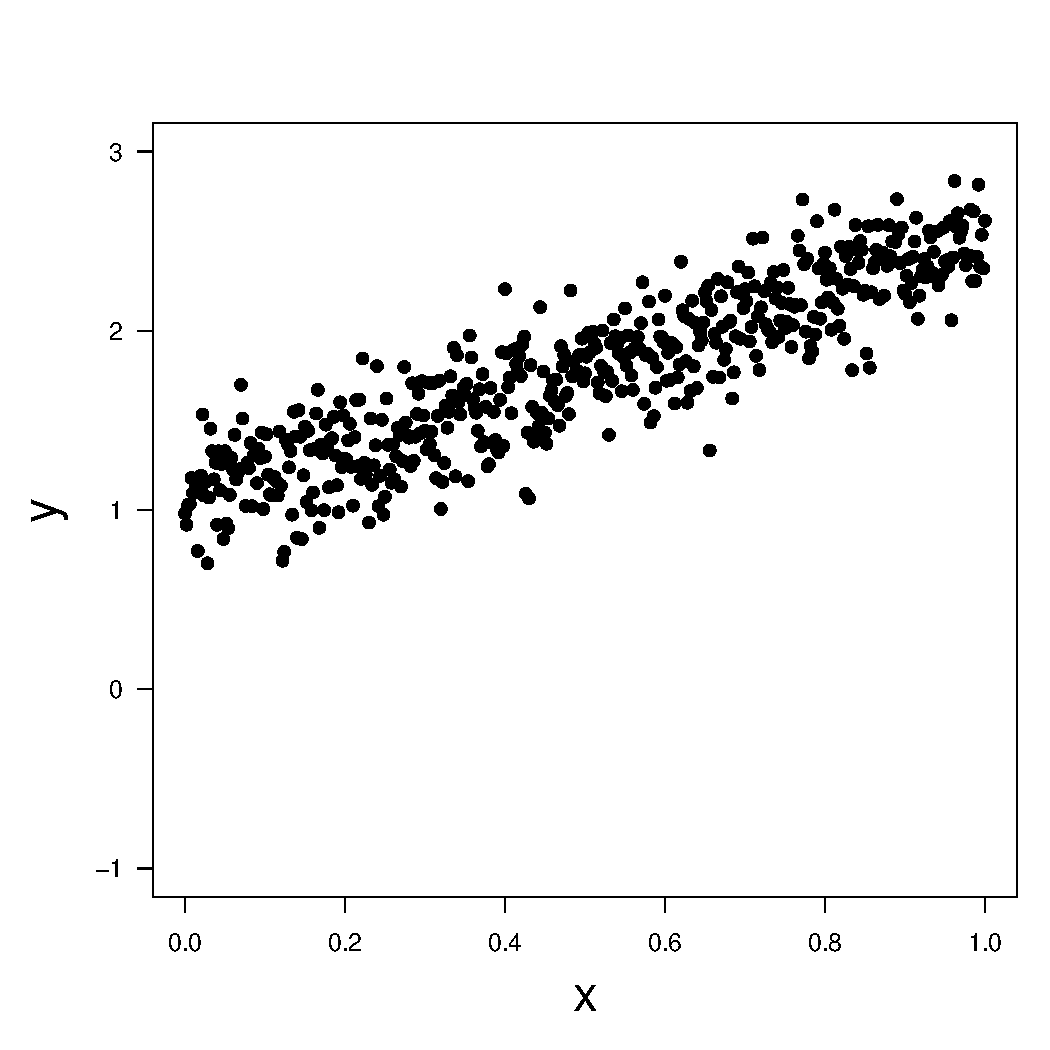
\includegraphics[width=10cm]{data.pdf}
\end{center}
We want to fit a straight line $y=\beta_0+\beta_1 x$ to the data points. We know the 
line has to make the resuduals having zero mean and zero correlation with $x_i$. 
First, let's imagine choosing various values of $\beta_1$ and see what the plot 
$y-\beta_1 x$ versus $x$ look like. In general, we will have the plot similar to the 
one above but with different overall slope. If we pick the right value of $\beta_1$, 
we will see that the residual $y-\beta_1 x$ vs $x$ is flat:  
\begin{center}
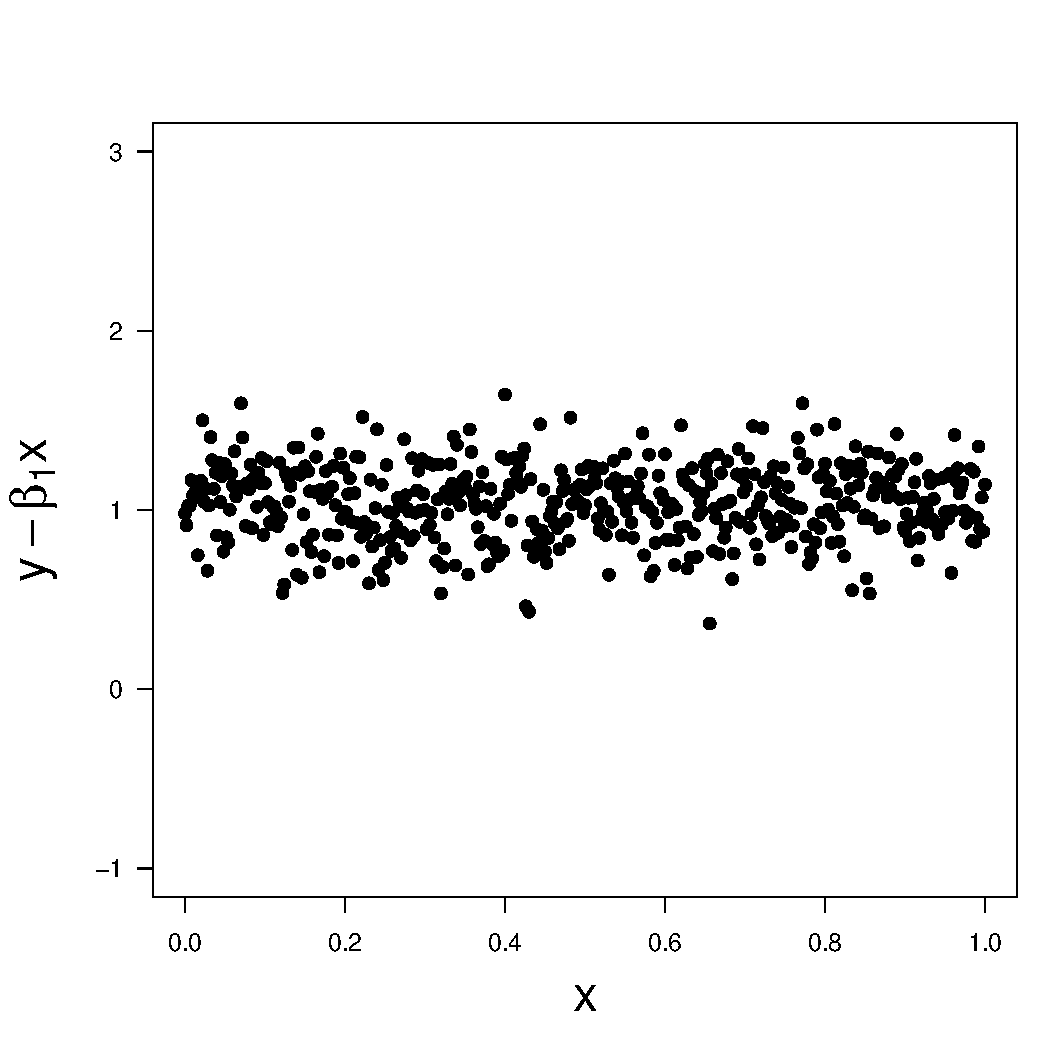
\includegraphics[width=10cm]{partial_residuals.pdf}
\end{center}
We know have achieved the first goal: by choosing the right value of $\beta_1$, 
the residual $y-\beta_1 x$ has zero correlation with $x$. However, the residuals 
do not have zero mean. So next we want to choose $\beta_0$ so that 
$y-\beta_0-\beta_1 x$ has zero mean. When the right value of $\beta_0$ is chosen, 
the residuals become this:
\begin{center}
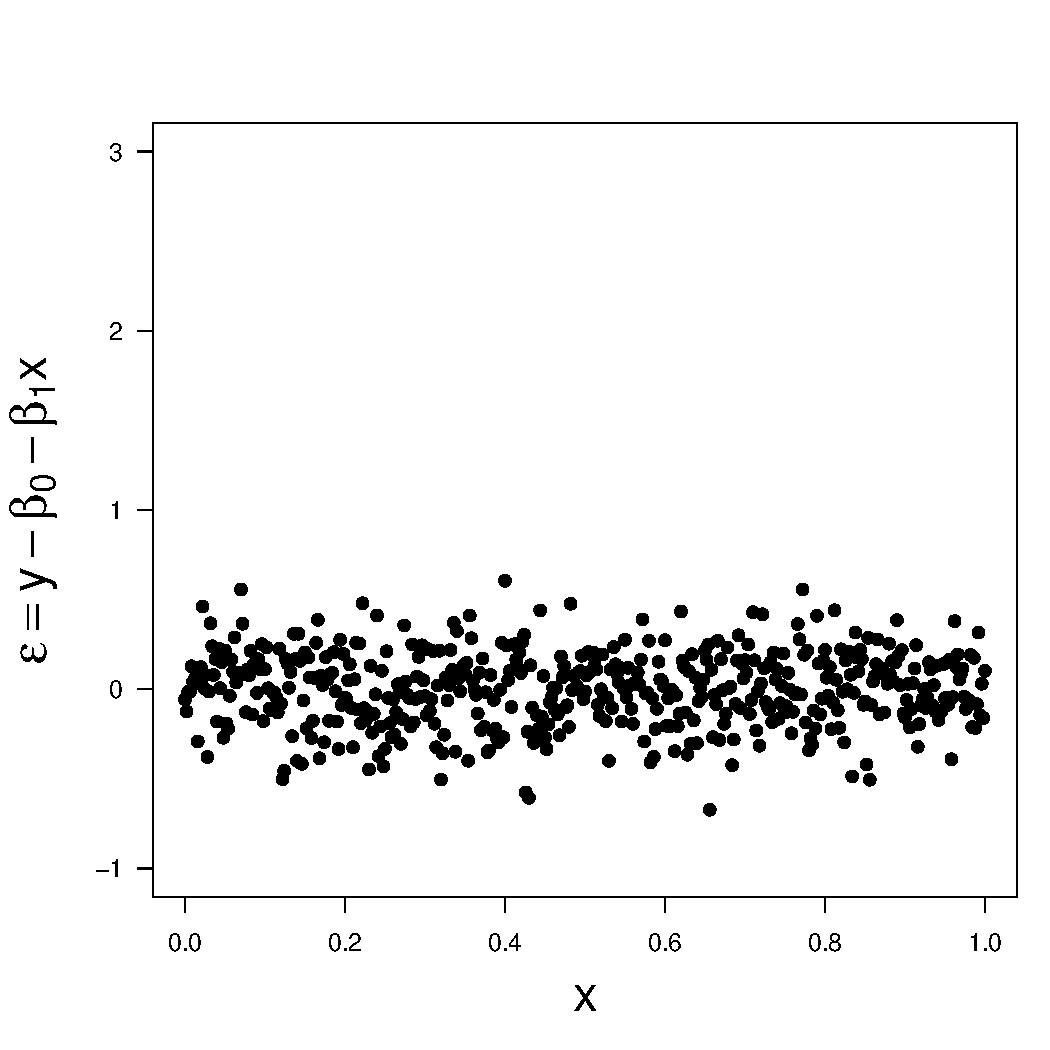
\includegraphics[width=10cm]{residuals.pdf}
\end{center}
We have accomplished our goal. The residuals now have zero mean and zero correlation 
with $x_i$. The resulting regression line $y=\beta_0+\beta_1x$ 
is the straight line that is best fit to the data points. The graph below 
shows the regression line (blue), data points (black) and the residuals (red). 
\begin{center}
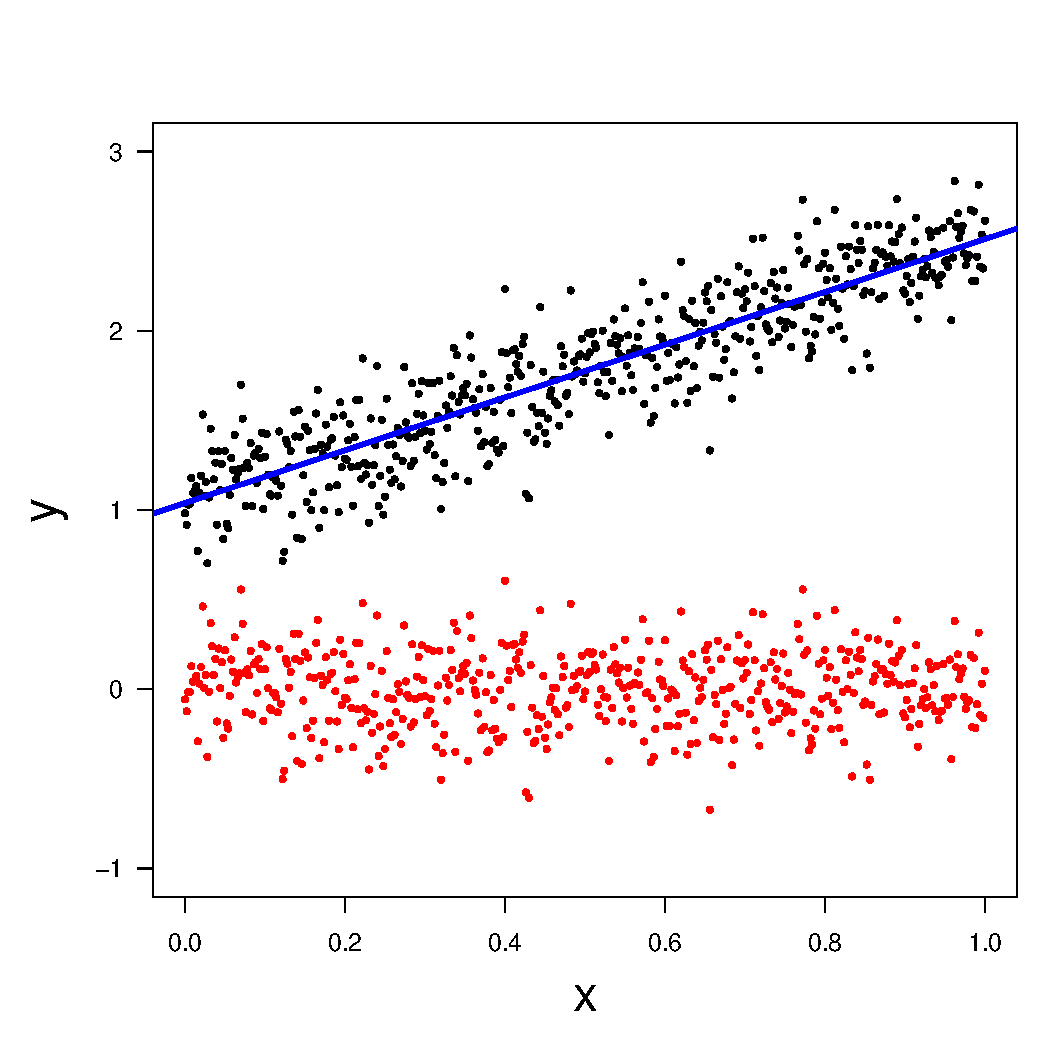
\includegraphics[width=10cm]{regressionLine.pdf}
\end{center}

We have outlined the idea of linear regression. Next we introduce the 
the concept of a vector, which proves to be very useful for regression 
with more than one variables.

\subsection{Vectors}

An $n$-dimensional vector $\ve{V}$ contains $n$ real numbers $v_1,v_2,\cdots,v_n$, often 
written in the form 
\[
  \ve{V} = \left( \begin{array}{c} v_1 \\ v_2 \\ \vdots \\ v_n \end{array} \right) 
\]
The numbers $v_1,v_2,\cdots,v_n$ are called the {\it components} of $\ve{V}$. 
Here we adopt the convention to write vector variables in boldface to distinguish 
them from numbers. It is useful to define a special vector $\ve{X_0}$ whose 
components are all equal to 1. That is, 
\beq
  \ve{X_0} = \left( \begin{array}{c} 1 \\ 1 \\ \vdots \\ 1 \end{array} \right)
\eeq
The scalar product of two vectors $\ve{U}$ and $\ve{V}$ is defined as 
\[
  \ve{U}\cdot \ve{V} = \ve{V} \cdot \ve{U} = \sum_{i=1}^n u_i v_i ,
\]
where $v_i$ and $u_i$ are components of $\ve{V}$ and $\ve{U}$. Note that the 
result of the scalar product of two vectors is a number, not a vector. 
Two vectors $\ve{U}$ and $\ve{V}$ are said to be {\it orthogonal} if  
$\ve{U}\cdot \ve{V}=0$. 

It follows from the definition that 
\[
  \ve{V} \cdot \ve{V} = \sum_{i=1}^n v_i^2 \geq 0 ,
\]
with $\ve{V}\cdot \ve{V}=0$ if and only if all components of $\ve{V}$ are 0. 
It follows from the Cauchy-Schwarz inequality that 
\[
  (\ve{U}\cdot \ve{V})^2 \leq (\ve{U}\cdot \ve{U}) (\ve{V} \cdot \ve{V}) 
\]
with the equality holds if and only if $\ve{U}=k\ve{V}$ for some constant $k$. 

Now that we have introduced the basic concept of a vector, we are now ready to 
express the regression equations in vector form.

\subsection{Regression Equations in Vector Form}

Equation~(\ref{def:residual}) can be written as 
\beq
  \ve{Y} = \ve{\hat{Y}} + \ve{\epsilon} = \beta_0 \ve{X_0} + \beta_1 \ve{X} + \ve{\epsilon} .
\label{vec:epsilon}
\eeq
The sum of square of residuals $SSE$ in~(\ref{def:SSE}) can be written as 
\beq
  SSE = \ve{\epsilon} \cdot \ve{\epsilon} = (\ve{Y}-\ve{\hat{Y}})\cdot (\ve{Y}-\ve{\hat{Y}}) 
= (\ve{Y}-\beta_0 \ve{X_0}-\beta_1 \ve{X})\cdot (\ve{Y}-\beta_0 \ve{X_0}-\beta_1 \ve{X}) 
\label{vec:SSE}
\eeq
To minimize $SSE$, we set the derivatives of $SSE$ with respect to $\beta_0$ and $\beta_1$ 
to 0. The resulting equations are 
\[
  \ve{X_0} \cdot (\ve{Y}-\beta_0 \ve{X_0}-\beta_1 \ve{X})=0 \ \ , \ \ 
  \ve{X} \cdot (\ve{Y}-\beta_0 \ve{X_0}-\beta_1 \ve{X})=0 
\]
or 
\beq
  \ve{X_0} \cdot \ve{\epsilon} = \ve{X} \cdot \ve{\epsilon} = 0 .
\label{vec:regeqs}
\eeq
This is equation~(\ref{eq:regeqs0}) written in vector form.
We see that the least square prescription can be interpreted as finding 
$\beta_0$ and $\beta_1$ to make the residual vector $\ve{\epsilon}$ orthogonal 
to both $\ve{X_0}$ and $\ve{X}$.

The mean and standard deviation in~(\ref{def:mean_std}) can be expressed as 
\beq
  \bar{u} = \frac{1}{n}\ve{X_0}\cdot \ve{U} \ \ , \ \ 
SD_u = \sqrt{\frac{1}{n} (\ve{U}-\bar{u}\ve{X_0})\cdot (\ve{U}-\bar{u}\ve{X_0})} 
\label{vec:mean_std}
\eeq
and the $Z$ score in (\ref{def:Zscore}) becomes 
\beq
  \ve{Z_u} = \frac{\ve{U}-\bar{u} \ve{X_0}}{SD_u} 
\label{vec:Zscore}
\eeq
It follows that 
\beq
  \ve{Z_u} \cdot \ve{Z_u} = n 
\label{vec:Znorm}
\eeq
The correlation $r_{xy}$ in~(\ref{def:correlation}) is proportional to the scalar product of $\ve{Z_x}$ 
and $\ve{Z_y}$: 
\beq
  r_{xy} = \frac{1}{n} \ve{Z_x} \cdot \ve{Z_y} 
\label{vec:correlation}
\eeq 
The equation $r_{x\epsilon}=0$ is equivalent to 
\beq
  \ve{Z_x} \cdot \ve{\epsilon} = 0
\eeq
We see that the equations in vector form are simpler and more elegant. We are now 
ready to solve the regression equations~(\ref{vec:epsilon}) and (\ref{vec:regeqs}) 
for $\beta_0$ and $\beta_1$.

\subsection{Regression Coefficients} 
\label{sec:regcoefs}

In this section, we are going to use the vector algebra to solve for $\beta_0$ and $\beta_1$ 
to re-derive equations~(\ref{eq:regcoefs0}). This is a useful exercise because it can be 
easily generalized to multiple regression we will consider later.

Start with equation~(\ref{vec:epsilon}). Taking the scalar product of~(\ref{vec:epsilon}) with 
$\ve{X_0}$, using equations~(\ref{vec:mean_std}), (\ref{vec:regeqs}) and $\ve{X_0}\cdot \ve{X_0}=n$, we obtain 
\beq
  n\bar{y} = n \beta_0 + n \beta_1 \bar{x} \ \ \ \Rightarrow \ \ \ 
  \bar{y} = \beta_0 + \beta_1 \bar{x} ,
\label{eq:bary2}
\eeq
Multiplying both sides of the above equation by 
$\ve{X_0}$ gives 
\[
  \bar{y} \ve{X_0} = \beta_0 \ve{X_0} + \beta_1 \bar{x} \ve{X_0} 
\]
Subtracting the above equation from~(\ref{vec:epsilon}) gives 
\[
  \ve{Y}-\bar{y} \ve{X_0} = \beta_1 (\ve{X}-\bar{x} \ve{X_0}) + \ve{\epsilon} 
\]
It follows from equation~(\ref{vec:Zscore}) that $\ve{Y}-\bar{y} \ve{X_0} = SD_y \ve{Z_y}$ 
and $\ve{X}-\bar{x} \ve{X_0} = SD_x \ve{Z_x}$.
%%\[
%%  \ve{Y}-\bar{y} \ve{X_0} = SD_y \ve{Z_y} \ \ \ \mbox{ and } \ \ \ 
%%  \ve{X}-\bar{x} \ve{X_0} = SD_x \ve{Z_x} .
%%\]
Hence we have 
\[
  SD_y \ve{Z_y} = \beta_1 SD_x \ve{Z_x} + \ve{\epsilon} 
\]
Taking the scalar product with $\ve{Z_x}$ and using $\ve{Z_x} \cdot \ve{\epsilon}=0$, we obtain 
\[
  SD_y \ve{Z_x} \cdot \ve{Z_y} =\beta_1 SD_x \ve{Z_x} \cdot \ve{Z_x} 
\]
It follows from equation~(\ref{vec:correlation}) and (\ref{vec:Znorm}) that 
$\ve{Z_x} \cdot \ve{Z_y}=n r_{xy}$ and $\ve{Z_x} \cdot \ve{Z_x}=n$ and so the 
above equation reduces to 
\[
  SD_y r_{xy} = \beta_1 SD_x \ \ \ \Rightarrow \ \ \ \beta_1 = r_{xy} \frac{SD_y}{SD_x} .
\]
Combining the above equation with~(\ref{eq:bary2}), we finally solve $\beta_0$ and $\beta_1$: 
\beq
  \boxed{ \beta_1 = r_{xy} \frac{SD_y}{SD_x} \ \ \ , \ \ \ 
  \beta_0 = \bar{y}-\beta_1 \bar{x} } 
\label{eq:regcoefs}
\eeq
The regression line is the straight line with slope $r_{xy} SD_y/SD_x$ passing 
through the point $(\bar{x},\bar{y})$.

\subsection{SST, SSM, SSE}
\label{sec:RMSE}

The total sum square $SST$ is defined as 
\beq
  SST = \sum_{i=1}^n (y_i-\bar{y})^2 = (\ve{Y}-\bar{y} \ve{X_0}) \cdot (\ve{Y}-\bar{y} \ve{X_0})
\label{def:SST}
\eeq
It follows from the definition of standard deviation [see equation~(\ref{def:mean_std}) 
or (\ref{vec:mean_std})] that 
\beq
  SST = n SD_y^2 
\label{eq:SST}
\eeq
The sum square predicted by the linear model $SSM$ is defined as 
\beq
  SSM = \sum_{i=1}^n (\hat{y}_i-\bar{y})^2 = (\ve{\hat{Y}}-\bar{y}\ve{X_0})\cdot (\ve{\hat{Y}}-\bar{y}\ve{X_0})
\label{def:SSM}
\eeq
Using $\ve{\hat{Y}}=\beta_0 \ve{X_0}+\beta_1 \ve{X}$ and $\beta_0=\bar{y}-\beta_1\bar{x}$, we have 
\beq
  \ve{\hat{Y}}-\bar{y}\ve{X_0} = (\bar{y}-\beta_1\bar{x})\ve{X_0}+\beta_1 \ve{X} - \bar{y}\ve{X_0} 
= \beta_1 (\ve{X}-\bar{x}\ve{X_0}) = \beta_1 SD_x \ve{Z_x} ,
\label{eq:hatY_baryX0}
\eeq
where we have used equation~(\ref{vec:Zscore}) to obtain the last equality. Combining~(\ref{def:SSM}), 
(\ref{eq:hatY_baryX0}), (\ref{vec:Znorm}) (\ref{eq:regcoefs}) and (\ref{eq:SST}), we obtain 
\beq
  SSM = n \beta_1^2 SD_x^2 = n \left( r_{xy} \frac{SD_y}{SD_x}\right)^2 SD_x^2 = n r_{xy}^2 SD_y^2 
= r_{xy}^2 SST 
\label{eq:SSM}
\eeq 
Next we want to prove the identity $SST=SSM+SSE$. To see that, we start with the identity 
\[
  \ve{Y}-\bar{y}\ve{X_0} = (\ve{Y}-\ve{\hat{Y}}) + (\ve{\hat{Y}}-\bar{y}\ve{X_0})  
= \ve{\epsilon} + (\ve{\hat{Y}}-\bar{y}\ve{X_0})
\]
We then ``square'' both sides by taking the scalar product with itself: 
\[
  (\ve{Y}-\bar{y}\ve{X_0})\cdot (\ve{Y}-\bar{y}\ve{X_0}) = [\ve{\epsilon} + (\ve{\hat{Y}}-\bar{y}\ve{X_0})] 
\cdot [\ve{\epsilon} + (\ve{\hat{Y}}-\bar{y}\ve{X_0})] 
\]
The left hand side is $SST$, the right hand side is the sum of $SSE$, $SSM$ and a cross term: 
\beqn
  SST &=& \ve{\epsilon} \cdot \ve{\epsilon} + (\ve{\hat{Y}}-\bar{y}\ve{X_0})\cdot (\ve{\hat{Y}}-\bar{y}\ve{X_0}) 
+ 2 \ve{\epsilon} \cdot (\ve{\hat{Y}}-\bar{y}\ve{X_0}) \cr 
&=& SSE + SSM + 2 \ve{\epsilon} \cdot (\ve{\hat{Y}}-\bar{y}\ve{X_0}) \nonumber
\eeqn
It follows from~(\ref{eq:hatY_baryX0}) and $\ve{Z_x}\cdot \ve{\epsilon}=0$ that the 
cross term vanishes:
\[
  \ve{\epsilon} \cdot (\ve{\hat{Y}}-\bar{y}\ve{X_0}) = \beta_1 SD_x \ve{Z_x}\cdot \ve{\epsilon}=0 
\]
Another way of seeing this is to note that $\ve{\epsilon}$ is orthogonal to both $\ve{X_0}$ and 
$\ve{X}$, as required by the least square prescription~(\ref{vec:regeqs}). 
So $\epsilon$ is orthogonal to any linear combination of $\ve{X_0}$ and $\ve{X}$. 
Since $\ve{\hat{Y}}-\bar{y}\ve{X_0}$ is a linear combination of $\ve{X_0}$ and $\ve{X}$, 
it is orthogonal to $\ve{\epsilon}$. 

We have just proved that 
\beq
  \boxed{ SST = SSM + SSE }
\label{eq:SSequality}
\eeq
We have calculated above that $SSM=r_{xy}^2 SST$ and $SST=n SD_y^2$. Using the identity $SST=SSM+SSE$, we 
obtain 
\[
  SSE = SST-SSM = (1-r_{xy}^2) SST = n (1-r_{xy}^2) SD_y^2 .
\]

\section{Multiple Regression} 

Now we want to generalize the results of simple regression to multiple regression. 
We will first consider the case with two variables in Section~\ref{sec:2vars}, 
because simple analytic expressions 
exist in this case and the derivation is relatively straightforward. 
Then we will turn to the more general case with more than two 
variables in Section~\ref{sec:multiVars}. 

\subsection{Two Variables}
\label{sec:2vars}

Suppose we want to fit the data points $\{ y_i \}$ with two variables $\{ x_{1i}\}$ and $\{ x_{2i}\}$ 
by a linear model 
\[
  y_i = \hat{y}_i + \epsilon_i  \ \ , \ \ 
i = 1,2,\cdots,n
\]
with 
\[
  \hat{y}_i = \beta_0 + \beta_1 x_{1i} + \beta_2 x_{2i} .
\]
The least square prescription is again to find $\beta_0$, $\beta_1$ and $\beta_2$ to 
minimize the sum square of the residuals: 
\[
  SSE = \sum_{i=1}^n \epsilon_i^2= \sum_{i=1}^n (y_i-\hat{y}_i)^2 
\]
As in the case of simple regression, it is more convenient to rewrite the above equations in 
vector form as follows: 
\beq
  \ve{Y} = \ve{\hat{Y}}+\ve{\epsilon} = \beta_0 \ve{X_0} + \beta_1 \ve{X_1} + \beta_2 \ve{X_2} + \ve{\epsilon}
\label{eq:Y2vars}
\eeq
\beq
  \ve{\hat{Y}}=\beta_0 \ve{X_0} + \beta_1 \ve{X_1} + \beta_2 \ve{X_2} 
\label{eq:Yhat_2vars}
\eeq
\beq
  SSE = \ve{\epsilon}\cdot \ve{\epsilon} = (\ve{Y}-\beta_0 \ve{X_0} - \beta_1 \ve{X_1} - \beta_2 \ve{X_2})\cdot 
(\ve{Y}-\beta_0 \ve{X_0} - \beta_1 \ve{X_1} - \beta_2 \ve{X_2}) 
\eeq
To employ the least square prescription, we set the derivatives of $SSE$ with respect to 
$\beta_0$, $\beta_1$ and $\beta_2$ to 0. The resulting equations are 
\beq
  \ve{X_0} \cdot \ve{\epsilon}=\ve{X_1}\cdot \ve{\epsilon} = \ve{X_2} \cdot \ve{\epsilon} = 0.
\label{eq:multiregs}
\eeq
That is to say that $\ve{\epsilon}$ is orthogonal to $\ve{X_0}$, $\ve{X_1}$ and $\ve{X_2}$. 
In other words, $\ve{\hat{Y}}$ is the vector $\ve{Y}$ projected onto the vector space spanned 
by $\ve{X_0}$, $\ve{X_1}$ and $\ve{X_2}$. 

For convenience, we denote $\ve{Z_1}$ and $\ve{Z_2}$ as the $Z$-score vectors associated 
with $\ve{X_1}$ and $\ve{X_2}$, respectively. That is, 
\beq
  \ve{Z_1} = \frac{\ve{X_1}-\bar{x}_1 \ve{X_0}}{SD_1} \ \ , \ \ 
  \ve{Z_2} = \frac{\ve{X_2}-\bar{x}_2 \ve{X_0}}{SD_2} \ \ ,
\eeq
where $SD_1$ and $SD_2$ are the standard deviation of $\{ x_{1i}\}$ and $\{ x_{2i}\}$, 
respectively. We see that $\ve{Z_1}$ is a linear combination of $\ve{X_0}$ and $\ve{X_1}$; 
$\ve{Z_2}$ is a linear combination of $\ve{X_0}$ and $\ve{X_2}$. Since $\ve{\epsilon}$ 
to orthogonal to $\ve{X_0}$, $\ve{X_1}$ and $\ve{X_2}$, it is orthogonal to $\ve{Z_1}$ 
and $\ve{Z_2}$ as well: 
\beq
  \ve{Z_1}\cdot \ve{\epsilon} = \ve{Z_2} \cdot \ve{\epsilon} = 0 .
\eeq
Recall that the mean of a vector $\ve{U}$ is $\bar{u}=\ve{X_0}\cdot \ve{U}/n$, 
and the correlation between $\ve{U}$ and $\ve{V}$ is $r_{uv}= \ve{Z_u}\cdot \ve{Z_v}/n$. 
Thus the orthogonality conditions of $\ve{\epsilon}$ mean that 
(1) $\ve{\epsilon}$ has zero mean, $\bar{\epsilon}=0$, and (2) $\ve{\epsilon}$  
has zero correlation
with both $\ve{X_1}$ and $\ve{X_2}$: $r_{\epsilon 1}=r_{\epsilon 2}=0$.

To solve the regression equations~(\ref{eq:multiregs}), we take the scalar product 
of equation~(\ref{eq:Y2vars}) with $\ve{X_0}$, resulting in the equation 
\beq
  \bar{y} = \beta_0 + \beta_1 \bar{x}_1 + \beta_2 \bar{x}_2 
\label{eq:b0_2vars}
\eeq
This means that the regression line passes through the average point $(\bar{x}_1,\bar{x}_2,\bar{y})$. 
Multiplying equation~(\ref{eq:b0_2vars}) by $\ve{X_0}$ yields 
\[
  \bar{y} \ve{X_0} = \beta_0 \ve{X_0} + \beta_1 \bar{x}_1 \ve{X_0} + \beta_2 \bar{x}_2 \ve{X_0}
\]
Subtracting the above equation from~(\ref{eq:Y2vars}) gives 
\[
  \ve{Y} - \bar{y} \ve{X_0} = \beta_1 (\ve{X_1}-\bar{x}_1\ve{X_0}) + \beta_2 (\ve{X_2}-\bar{x}_2\ve{X_0}) 
+ \ve{\epsilon}
\]
Using the definition of the $Z$ score vector, we can write the above equation as 
\beq
  SD_y \ve{Z_y} = \beta_1 SD_1 \ve{Z_1} + \beta_2 SD_2 \ve{Z_2} + \ve{\epsilon}
\label{eq:ZyZ1Z2}
\eeq
Taking the scalar product of the above equation with $\ve{Z_1}$ gives 
\beq
  SD_y r_{y1} = \beta_1 SD_1 + \beta_2 SD_2 r_{12} ,
\label{eq:tmp1}
\eeq
where $r_{y1}=\ve{Z_y}\cdot \ve{Z_1}/n$ is the correlation between $\ve{Y}$ and 
$\ve{X_1}$, $r_{12}=\ve{Z_1}\cdot \ve{Z_2}/n$ is the correlation between 
$\ve{X_1}$ and $\ve{X_2}$. Equation~(\ref{eq:tmp1}) can be written as 
\beq
  \beta_1 = r_{y1} \frac{SD_y}{SD_1} - \beta_2 \left( r_{12} \frac{SD_2}{SD_1}\right) 
= \beta_{y1} - \beta_2 \beta_{21} , 
\label{eq:beta1}
\eeq
where 
$\beta_{y1}= r_{y1} SD_y/SD_1$ is the slope in the simple regression for predicting $\ve{Y}$ 
from $\ve{X_1}$, and $\beta_{21}=r_{12} SD_2/SD_1$ is the slope in the simple regression 
for predicting $\ve{X_2}$ from $\ve{X_1}$. 

Before deriving the final expression for $\beta_1$, let's point out two things. First, 
if $r_{12}=0$ (or equivalently $\ve{X_1}\cdot \ve{X_2}=0$) then $\beta_1=\beta_{y1}$. 
That is to say that if the correlation bteween $\ve{X_1}$ and $\ve{X_2}$ is zero (orthogonal), 
the slope $\beta_1$ in the multiple regression is exactly the same as the slope 
$\beta_{y1}$ in the simple regression for prediction $\ve{Y}$ from $\ve{X_1}$. The 
addition of the $\ve{X_2}$ does not change the slope. Second, if $r_{12}>0$ and 
$\beta_2>0$, then $\beta_1 < \beta_{y1}$. The slope $\beta_1$ decreases if 
$\ve{X_1}$ and $\ve{X_2}$ are positively correlated and if the slope of $\ve{X_2}$ 
in the multiple regression is positive. 

Let's go back to equation~(\ref{eq:beta1}). If $r_{12} \neq0$, the equation of 
$\beta_1$ involves $\beta_2$. So $\beta_1$ and $\beta_2$ has to be solved 
together. Since $\ve{X_1}$ and $\ve{X_2}$ are symmetric, the equation for 
$\beta_2$ can be obtained by simply exchanging the index between 1 and 2 of 
the $\beta_1$ equation: 
\beq
  \beta_2 = \beta_{y2} - \beta_1 \beta_{12} ,
\label{eq:beta2}
\eeq
where 
\beq
  \beta_{y2} = r_{y2} \frac{SD_y}{SD_2} \ \ \mbox{ and } \ \ \beta_{12} = r_{12} \frac{SD_1}{SD_2} .
\eeq
Substituting $\beta_2$ from~(\ref{eq:beta2}) into~(\ref{eq:beta1}), we obtain 
\beq
  \beta_1 = \beta_{y1} - (\beta_{y2} - \beta_1 \beta_{12}) \beta_{21} 
= \beta_{y1} - \beta_{y2} \beta_{21} + \beta_1 \beta_{12} \beta_{21} 
\label{eq:tmp2}
\eeq
Note that the product 
\[
  \beta_{12} \beta_{21} = \left( r_{12} \frac{SD_1}{SD_2}\right) \left( r_{12}\frac{SD_2}{SD_1}\right) 
= r_{12}^2 .
\]
Thus equation~(\ref{eq:tmp2}) becomes 
\[
  \beta_1 = \beta_{y1} - \beta_{y2} \beta_{21} + r_{12}^2 \beta_1 \ \ \ \Rightarrow \ \ \
  (1-r_{12}^2) \beta_1 = \beta_{y1} - \beta_{y2} \beta_{21} 
\]
or 
\[
  \beta_1 = \frac{\beta_{y1} - \beta_{y2} \beta_{21}}{1-r_{12}^2} 
\]
Using the expressions for $\beta_{y1}$, $\beta_{y2}$ and $\beta_{12}$, we find 
\beq
  \beta_1 = b_1 \frac{SD_y}{SD_1} , 
\label{eq:beta1_2vars}
\eeq
where 
\[
  b_1 = \frac{r_{y1}-r_{y2} r_{12}}{1-r_{12}^2} 
\]
may be interpreted as the adjusted correlation between $\ve{Y}$ and $\ve{X_1}$ 
taking into account the presence of $\ve{X_2}$.
The expression for $\beta_2$ is obtained by exchanging 
the index between 1 and 2: 
\[
  \beta_2 = b_2 \frac{SD_y}{SD_2} \ \ , \ \ b_2 = \frac{r_{y2}-r_{y1} r_{12}}{1-r_{12}^2} .
\]
Gathering all the results, we conclude that the regression coefficients are given by 
\beq
  \boxed{ \beta_1 = b_1 \frac{SD_y}{SD_1} \ \ , \ \ \beta_2=b_2 \frac{SD_y}{SD_1} \ \ , \ \ 
  \beta_0 = \bar{y}-\beta_1 \bar{x}_1 - \beta_2 \bar{x}_2 }
\label{eq:regcoefs2vras}
\eeq
with 
\beq
  \boxed{ b_1 = \frac{r_{y1}-r_{y2} r_{12}}{1-r_{12}^2} \ \ , \ \ 
  b_2 = \frac{r_{y2}-r_{y1} r_{12}}{1-r_{12}^2} }
\label{eq:b1b2}
\eeq

In Section~\ref{sec:RMSE}, we see that the SSE in simple regression is related 
to $SD_y^2$ by 
$SSE = n(1-r_{xy}^2)\, SD_y^2$. In multiple regression, we will show 
in Section~\ref{sec:RMSE_multi} that the formula is generalized to 
\[
  SSE = n^2(1-R^2)\, SD_y^2 ,
\]
where $R$ is the correlation between $\ve{Y}$ and $\ve{\hat{Y}}$: 
\[
  R = \frac{\ve{Z_y} \cdot \ve{Z_{\hat{y}}}}{n}  \ .
\]
We will defer the calculation of $R$ to Section~\ref{sec:R_multi}. 
In the case of multiple regression with two variables considered here, 
$R$ is given by 
\beq
  \boxed{ R = \sqrt{ \frac{r_{y1}^2 +r_{y2}^2 - 2r_{y1}r_{y2} r_{12}}{1-r_{12}^2}} }
\label{eq:R_2vars}
\eeq

\subsection{More Than Two Variables}
\label{sec:multiVars}

Suppose we now want to fit $\{ y_i \}$ with $p$ variables 
$\{x_{1i}, x_{2i}, \cdots, x_{pi} \}$. The regression equation 
has $p+1$ parameters $\beta_0,\beta_1,\beta_2,\cdots, \beta_p$. 
It can be written in the vector form as 
\beq
  \ve{Y} = \ve{\hat{Y}} + \ve{\epsilon} = \sum_{j=0}^p \beta_j \ve{X_j} + \ve{\epsilon} 
\label{eq:epsilon_multi}
\eeq
\beq
  \ve{\hat{Y}} = \sum_{j=0}^p \beta_j \ve{X_j} 
\label{eq:Yhat_multi}
\eeq
\beq
  SSE = \ve{\epsilon} \cdot \ve{\epsilon} = \left( \ve{Y} - \sum_{j=0}^p \beta_j \ve{X_j} 
\right) \cdot \left( \ve{Y} - \sum_{j=0}^p \beta_j \ve{X_j} \right) 
\label{eq:SSE_multi}
\eeq
To minimize $SSE$, we set the derivatives of $SSE$ with respect to 
$\beta_j$ $(j=0,1,\cdots,p)$ to 0. The resulting equations can be written as 
\beq
  \ve{X_j} \cdot \ve{\epsilon} = 0 \ \ \ , \ \ j=0,1,\cdots, p.
\label{eq:regres_multi}
\eeq
This means that $\ve{\epsilon}$ is orthogonal all $\ve{X_0},\ve{X_1},\cdots,\ve{X_p}$, 
or equivalently, the mean of $\ve{\epsilon}$ is 0 and the correlations 
between $\ve{\epsilon}$ and all the X variables are 0. 

To find the regression coefficients, we follow the same procedures as before. 
First, take the scalar product of equation~(\ref{eq:epsilon_multi}) with $\ve{X_0}$. 
The result is 
\beq
  \bar{y} = \beta_0 + \sum_{j=1}^p \beta_j \bar{x}_j 
\label{eq:bary_multi}
\eeq
As before, this means that the regression line passes through the point of 
average. Next, we multiple the above equation by $\ve{X_0}$: 
\[
  \bar{y} \ve{X_0} = \beta_0 \ve{X_0} + \sum_{j=1}^p \beta_j \bar{x}_j \ve{X_0} 
\]
and then subtract it from equation~(\ref{eq:epsilon_multi}):
\[
  \ve{Y} - \bar{y} \ve{X_0} = \sum_{j=1}^p \beta_j (\ve{X_j}-\bar{x}_j \ve{X_0}) 
+ \ve{\epsilon} \ .
\]
Using the definition of the $Z$ score vector~(\ref{vec:Zscore}), we can 
write the above equation as 
\[
   SD_y \ve{Z_y} = \sum_{j=1}^p \beta_j SD_j \ve{Z_j} + \ve{\epsilon} .
\]
Dividing both sides by $SD_y$ results in 
\beq
  \ve{Z_y} = \sum_{j=1}^p b_j \ve{Z_j} + \frac{\ve{\epsilon}}{SD_y} ,
\label{eq:Zy_multi}
\eeq
where 
\beq
  b_j = \beta_j \frac{SD_j}{SD_y} .
\label{def:bj}
\eeq
Taking the scalar product of equation~(\ref{eq:Zy_multi}) with $\ve{Z_i}$ 
$(i=0,1,2,\cdots,p)$, we obtain 
\beq
  \sum_{j=1}^p r_{ij} b_j = r_{yi} \ \ , \ \ i=1,2,\cdots, p. 
\label{eq:beqs}
\eeq
This is a system of linear equations for $b_1,b_2,\cdots,b_p$. Written them out, 
they look like 
\beqn
  b_1 + r_{12} b_2 + r_{13} b_3 + \cdots + r_{1p} b_p &=& r_{y1} \cr 
  b_1 r_{21} + b_2 + r_{23} b_3 + \cdots + r_{2p} b_p &=& r_{y2} \cr 
  b_1 r_{31} + b_2 r_{32} + b_3 + \cdots + r_{3p} b_p &=& r_{y3} \cr 
  \vdots & \vdots & \vdots \cr 
  b_1 r_{p1} + b_2 r_{p2} + b_3 r_{p3} + \cdots + b_p &=& r_{yp} \nonumber 
\eeqn
If all of the variables $\ve{X_j}$ are uncorrelated (i.e.\ $r_{ij}=0$ 
if $i\neq j$), the solution is $b_j=r_{yj}$ and the slopes are 
$\beta_j=r_{yj} SD_y/SD_j$. This is exactly the same as the slopes 
in simple regression for predicting $\ve{Y}$ from $\ve{X_j}$. 

There are no simple analytic expressions for $b_j$ in general, but 
there are several well-known procedures to obtain the solution by successive 
algebraic operations, but we will not discuss the methods here.

Suppose all the $b$'s have been solved using one of those 
procedures, the slopes are given by equation~(\ref{def:bj}) as 
\beq
  \beta_j = b_j \frac{SD_j}{SD_y}  \ \ , \ \ j=1,2,\cdots, p 
\label{eq:slopes_multi}
\eeq
and the intercept $\beta_0$ is given by equation~(\ref{eq:bary_multi}) as 
\beq
  \beta_0 = \bar{y} - \sum_{j=1}^p \beta_j \bar{x}_j .
\label{eq:intercept_multi}
\eeq

Finally, we should mention that the term ``linear'' in linear regession 
refers to a model being linear in the fitting parameters 
$\beta_0,\beta_1,\cdots,\beta_p$. For example, we can fit $y_i$ by the 
model 
\beq
  y_i = \beta_0 + \beta_1 x_i + \beta_2 \sqrt{x_i} + \beta_3 x_i^2 + \beta_4 \ln x_i 
+ \beta_5 \frac{x_i^3}{1+2^{x_i}}
\label{eq:nonlinearX}
\eeq
using the technique of multiple linear regression since the model is 
linear in $\beta_0,\beta_1,\cdots,\beta_5$. We simply label 
\[
  x_{1i} = x_i \ \ , \ \ x_{2i}=\sqrt{x_i} \ \ , \ \ x_{3i}=x_i^2 \ \ , \ \ 
  x_{4i}=\ln x_i \ \ , \ \ x_{5i}= \frac{x_i^3}{1+2^{x_i}}
\]
and equation~(\ref{eq:nonlinearX}) can be written in vector form as 
\[
  \ve{Y}=\beta_0 \ve{X_0} + \beta_1 \ve{X_1} + \beta_2 \ve{X_2} + \beta_3 \ve{X_3} 
+ \beta_4 \ve{X_4} + \beta_5 \ve{X_5} \ ,
\]
which is equation~(\ref{eq:epsilon_multi}) with $p=5$. The key is to note that 
the least square prescription is to minimize $SSE$ by varying the paremeters 
$\beta$'s, not the independent variables $x$'s.

\subsection{Correlation Between $\ve{Y}$ and $\ve{\hat{Y}}$}
\label{sec:R_multi}

To generalize the SST, SSM, and SSE expressions in Section~\ref{sec:RMSE} for multiple 
regression, we 
consider the quantity $R$ defined as the correlation between $\ve{Y}$ and 
$\ve{\hat{Y}}$: 
\beq
 R = \frac{\ve{Z_y} \cdot \ve{Z_{\hat{y}}}}{n}  \ .
\label{def:R}
\eeq
We first calculate the average of $\ve{\hat{Y}}$: 
\[
  \bar{\hat{y}} = \frac{1}{n} \ve{\hat{Y}} \cdot \ve{X_0} 
= \frac{1}{n} \left( \beta_0 \ve{X_0} + \sum_{j=1}^p \beta_j \ve{X_j}\right) 
\cdot \ve{X_0} 
= \beta_0 + \sum_{j=1}^p \beta_j \bar{x}_j = \bar{y} ,
\]
where we have used equation~(\ref{eq:Yhat_multi}) for $\ve{\hat{Y}}$ and 
(\ref{eq:bary_multi}) for $\bar{y}$. From the definition of the $Z$ score 
vector~(\ref{vec:Zscore}) and $\bar{\hat{y}}=\bar{y}$, we can write~(\ref{def:R}) as 
\beqn
  R &=& \frac{(\ve{Y}-\bar{y} \ve{X_0})\cdot (\ve{\hat{Y}}-\bar{y} \ve{X_0})} 
{n SD_y SD_{\hat{y}}}  \cr \cr 
  &=& \frac{(\ve{\hat{Y}}+\ve{\epsilon}-\bar{y} \ve{X_0})\cdot (\ve{\hat{Y}}-\bar{y} \ve{X_0})}
{n SD_y SD_{\hat{y}}}  \cr \cr 
&=& \frac{(\ve{\hat{Y}}-\bar{y} \ve{X_0})\cdot (\ve{\hat{Y}}-\bar{y} \ve{X_0})}
{n SD_y SD_{\hat{y}}}  \cr \cr 
&=& \frac{SD_{\hat{y}}}{SD_y} 
\label{eq:R}
\eeqn
where we have used $\ve{\epsilon}\cdot \ve{X_0}=0$ and $\ve{\epsilon}\cdot \ve{\hat{Y}}=0$ 
(since $\ve{\hat{Y}}$ is a linear combination of $\ve{X_0},\cdots \ve{X_p}$ and all 
are orthogonal to $\ve{\epsilon}$). We have also used the definition of the 
standard deviation~(\ref{vec:mean_std}) to obtain the last line. Hence we have 
\beq
  R^2 = \frac{SD_{\hat{y}}^2}{SD_y^2} = \frac{\sum\limits_{i=1}^n (\hat{y}_i-\bar{y})^2}
{\sum\limits_{i=1}^n (y_i-\bar{y})^2} \ ,
\label{eq:R2}
\eeq
which is interpreted as the fraction of the variance of $\ve{Y}$ explained by 
the linear model.

To compute $R$, we use equation~(\ref{eq:Yhat_multi}) for $\ve{\hat{Y}}$ and 
(\ref{eq:intercept_multi}) for $\beta_0$, and write 
\beqn
  SD_{\hat{y}}^2 &=& \frac{1}{n} (\ve{\hat{Y}}-\bar{y} \ve{X_0})\cdot 
(\ve{\hat{Y}}-\bar{y} \ve{X_0}) \cr \cr 
&=& \frac{1}{n}\left[ (\beta_0-\bar{y}) \ve{X_0} + \sum_{i=1}^p \beta_i \ve{X_i}\right] \cdot 
\left[ (\beta_0-\bar{y}) \ve{X_0} + \sum_{j=1}^p \beta_j \ve{X_j}\right] \cr \cr 
&=&\frac{1}{n} \left[ \sum_{i=1}^p \beta_i (\ve{X_i}-\bar{x}_i \ve{X_0})\right] \cdot 
\left[ \sum_{j=1}^p \beta_j (\ve{X_j}-\bar{x}_j \ve{X_0})\right] \cr \cr 
&=&\frac{1}{n} \left( \sum_{i=1}^p SD_i \beta_i \ve{Z_i}\right) \cdot 
\left( \sum_{j=1}^p SD_j \beta_j \ve{Z_j}\right) \cr \cr 
&=&\frac{1}{n} \sum_{i=1}^p \sum_{j=1}^p SD_i SD_j \beta_i \beta_j  \ve{Z_i}\cdot \ve{Z_j} \cr \cr 
&=& \sum_{i=1}^p \sum_{j=1}^p SD_i SD_j \beta_i \beta_j r_{ij} \nonumber
\eeqn
\[
  R^2 = \frac{SD_{\hat{y}}^2}{SD_y^2} = \sum_{i=1}^p \sum_{j=1}^p b_i b_j r_{ij} ,
\]
where we have used the definition of $b_j$ in equation~(\ref{def:bj}). The sum 
can be simplified by noting that $b_j$ satisfy equation~(\ref{eq:beqs}), and thus 
we obtain 
\beq
  \boxed{ R = \sqrt{\sum_{i=1}^p b_i r_{yi} } }
\label{eq:Rgen}
\eeq
When the solution of $b_i$ is obtained, $R$ can be calculated using the above equation. 
In the case of multiple regression with two variables ($p=2$), $b_1$ and $b_2$ 
are given by equation~(\ref{eq:b1b2}). Plugging them into equation~(\ref{eq:Rgen}), 
we obtain equation~(\ref{eq:R_2vars}).

\subsection{SST, SSM, SSE}
\label{sec:RMSE_multi}

As in Section~\ref{sec:RMSE}, we define $SST$ and $SSM$ as 
\[
  SST = \sum_{i=1}^n (y_i-\bar{y})^2 = (\ve{Y}-\bar{y} \ve{X_0}) \cdot (\ve{Y}-\bar{y} \ve{X_0})
\]
\[
 SSM = \sum_{i=1}^n (\hat{y}_i-\bar{y})^2 = (\ve{\hat{Y}}-\bar{y}\ve{X_0})\cdot (\ve{\hat{Y}}-\bar{y}\ve{X_0})
\]
It follows from the definition of standard deviation that 
\beq
  SST = n SD_y^2 
\label{eq:SST_multi}
\eeq
and it follows from~(\ref{eq:R2}) that 
\beq
  SSM = R^2 SST .
\label{eq:SSM_multi}
\eeq
The identity $SST=SSM+SSE$ still holds in muiltiple linear regression. The proof 
is almost exactly the same as in Section~\ref{sec:RMSE}. 

We start with the identity 
\[
  \ve{Y}-\bar{y} \ve{X_0} = (\ve{Y}-\ve{\hat{Y}}) + (\ve{\hat{Y}}-\bar{y}\ve{X_0}) 
= \ve{\epsilon} + (\ve{\hat{Y}}-\bar{y}\ve{X_0}) .
\]
Take the scalar product with itself:
\beqn
  (\ve{Y}-\bar{y} \ve{X_0})\cdot (\ve{Y}-\bar{y} \ve{X_0}) &=& 
  [\ve{\epsilon} + (\ve{\hat{Y}}-\bar{y}\ve{X_0})]\cdot 
[\ve{\epsilon} + (\ve{\hat{Y}}-\bar{y}\ve{X_0})] \cr 
SST &=& SSE + SSM + 2 \ve{\epsilon} \cdot (\ve{\hat{Y}}-\bar{y}\ve{X_0})  
\nonumber
\eeqn
Since $\ve{\hat{Y}}-\bar{y}\ve{X_0}$ is a linear combination of 
$\ve{X_0},\ve{X_1},\cdots, \ve{X_p}$ and $\ve{\epsilon}$ is orthogonal 
to all these vectors, $\epsilon \cdot (\ve{\hat{Y}}-\bar{y}\ve{X_0})=0$ and 
so we have 
\beq
  \boxed{ SST = SSM + SSE} 
\label{eq:SSTequality_multi} 
\eeq

\end{document}
